\documentclass
   [kulak] % options: kulak (default) or kul, handout 
   {kulakbeamer}

\usepackage[dutch]{babel}
\usepackage[T1]{fontenc}
\usepackage{graphicx}

\title[Smart Fire Extinguisher]{Smart Fire Extinguisher - Tussentijdse Presentatie}
\subtitle{Teamopdracht P\&O}
\author[Team 6]{TEAM 6: Anna-Laura, Emile, Jérôme, Jesse} 
\institute[Kulak]{KU Leuven Kulak}
\date{Academiejaar 2022 -- 2023}

%% Overview at begin of each section; delete if unwanted.
\AtBeginSection[]{
	\begin{frame}
	\frametitle{Overzicht} %Change to "Outline" for English presentation
	{
		\hypersetup{hidelinks} %disable link colors
		\hfill	{\large\parbox{.95\textwidth}{\tableofcontents[currentsection,hideothersubsections]}}
	}
\end{frame}}

\begin{document}

\begin{titleframe}
\titlepage
\end{titleframe}

\begin{outlineframe}[Overzicht]
\tableofcontents
\end{outlineframe}

 % % % Here you go  % % % 
 %------------------------------------------------------------%

\section{Inleiding}

\begin{frame}
\frametitle{Sprinklers} 

\begin{column}{ 0.5 \textwidth}
	{\bf{Voordelen}}\\[.2cm]
	\begin{itemize}
		\item Grote brandveiligheid
		\item Snelle interventie
		\item Volledig automatisch
	\end{itemize}
	{\bf{Nadelen}}\\[.2cm]
	\begin{itemize}
		\item Dure aanleg van waterleidingen
		\item Duur onderhoud van waterleidingen
		\item Bij defecten mogelijks grote schade 
	\end{itemize}
\end{column}
\begin{column}{ 0.5 \textwidth}
	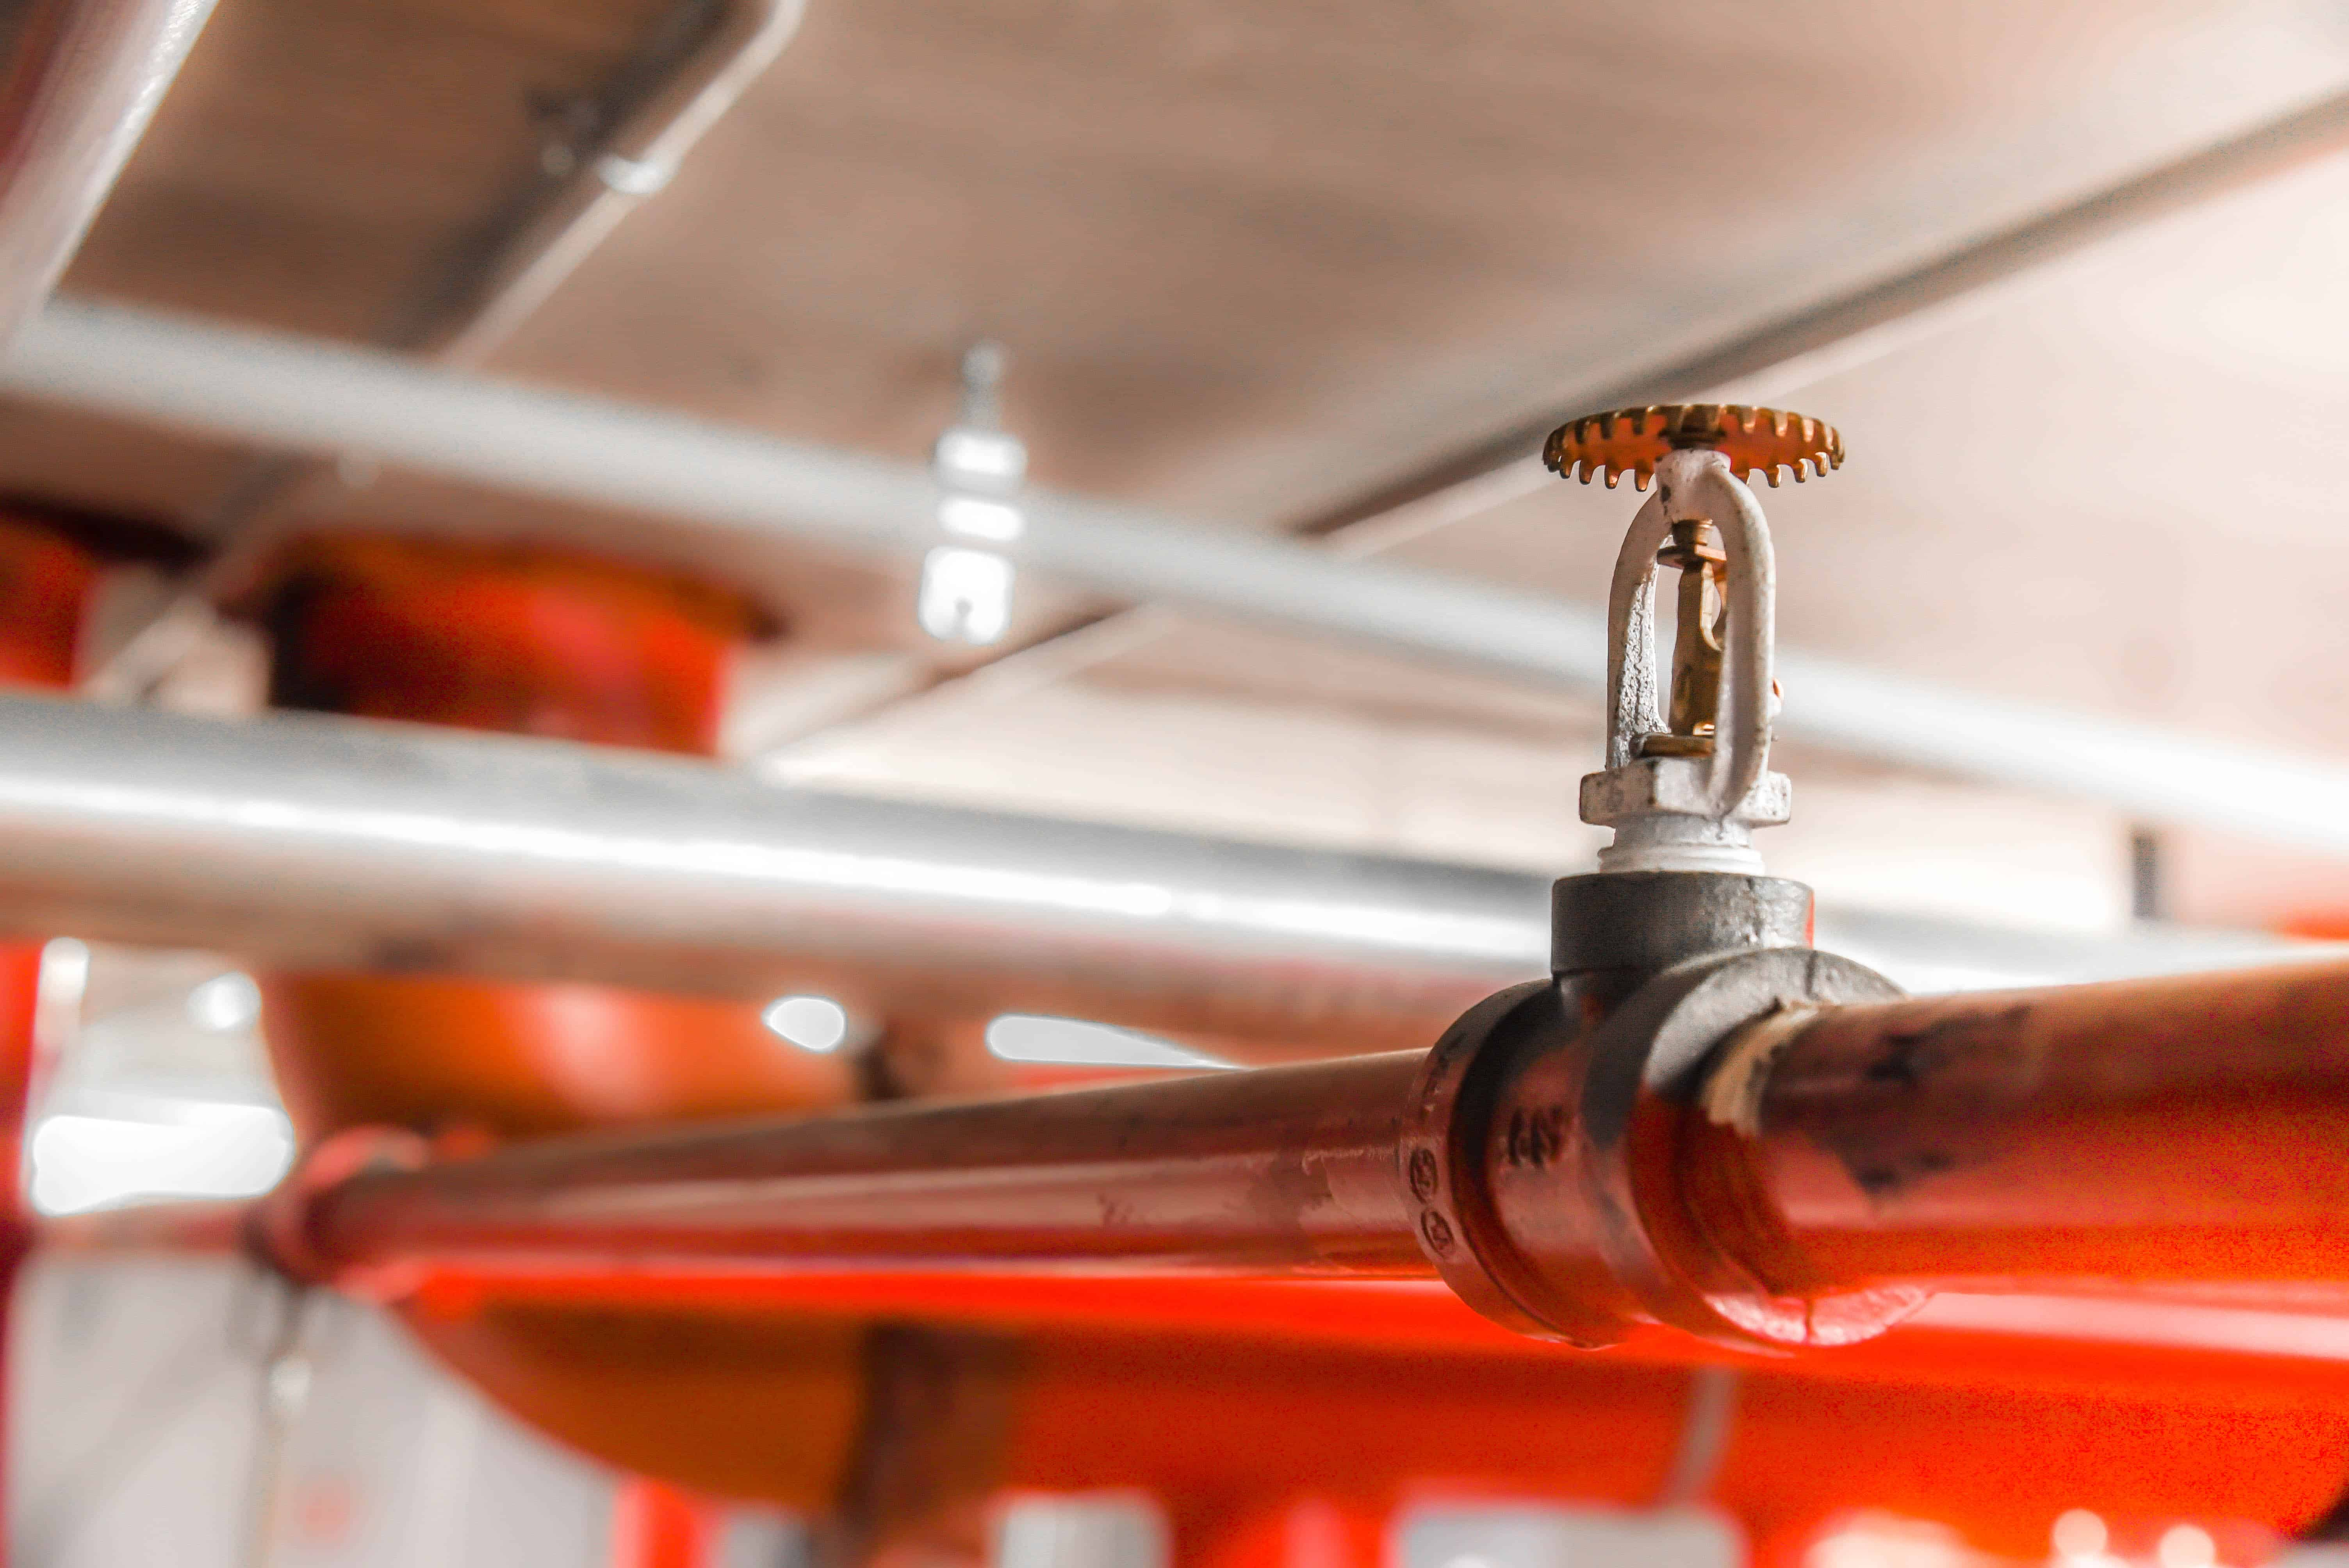
\includegraphics[width=0.8\textwidth]{sprinkler_foto_BEAMER}
\end{column}
\end{frame}

\begin{frame}
\frametitle{Oplossing}
{\bf{Stationair brandblusapparaat}}\\[.2cm]
\begin{itemize}
	\item Detecteert en localiseert de brand
	\item 

\end{frame}





\section[Ontwerp]{Ontwerp, Werking en Materiaal}

\begin{frame}
\frametitle{Klantenvereisten en ontwerpspecificaties}
Tekst.
\end{frame}

\begin{frame}
\frametitle{Ontwerp}
\end{frame}

\begin{frame}
\frametitle{Werking}
\end{frame}





\section{Besluit}
\begin{frame}
\frametitle{Wat hebben we al gerealiseerd?}
\end{frame}

\begin{frame}
\frametitle{Wat moet nog afgewerkt worden?}

\end{frame}

\begin{frame}
\frametitle{Bibliografie}
\bibliography{}
\end{frame}

\end{document}
